% NOTE: There are a couple of  commands that I used to make
% things align properly in my PDF. You should delete these when
% reformatting.



\chapter{Probability}


We use probability to describe uncertain events. When you accidentally
drop a slice of bread, you don't know if it's going to fall with the
buttered side facing upwards or downwards. When your favourite sports
team plays a game, you don't know whether they will win or not. When
the weatherman says that there is a $40\%$ chance of rain tomorrow, you
may or may not end up getting wet.  Uncertainty presents itself to
some degree in every event that occurs around us and in every decision
that we make.\par

We will see in this chapter that all of these uncertainties can be
described using the rules of probability theory and that we can make
definite conclusions about uncertain processes.\par

We'll use three examples of uncertain processes to help you understand
the meanings of the different words used in probability theory: tossing
a coin, rolling dice, and a soccer match.

\chapterstartvideo{VMbxk}

\Definition{Experiment}{An experiment refers to an uncertain process.}

\Definition{Outcome}{An outcome of an experiment is a single
  result of that experiment.}

\begin{figure}[H]
\textbf{Experiment 1} A coin is tossed and it lands with either
  heads (H) or tails (T) facing upwards. An example outcome of tossing
  a coin is that it lands with heads facing up:
  \begin{center}
    \begin{tikzpicture}
      \coinheads
    \end{tikzpicture}
  \end{center}
%   \caption{An example outcome of tossing a coin: it lands with heads
%     facing up.}
\end{figure}

\begin{figure}[H]
  \textbf{Experiment 2} Two dice are rolled and the total number of
  dots added up. An example outcome of rolling two dice:

  \begin{center}
    \begin{tikzpicture}
      \makedie{3}{shift={(-1,0)},rotate=10}
      \makedie{5}{shift={(1,0)},rotate=-20}
    \end{tikzpicture}
  \end{center}
%   \caption{An example outcome of rolling two dice.}
\end{figure}

\begin{figure}[H]
  \textbf{Experiment 3} Two teams play a soccer match and we are
  interested in the final score. An example outcome of a soccer match:

  \begin{center}
    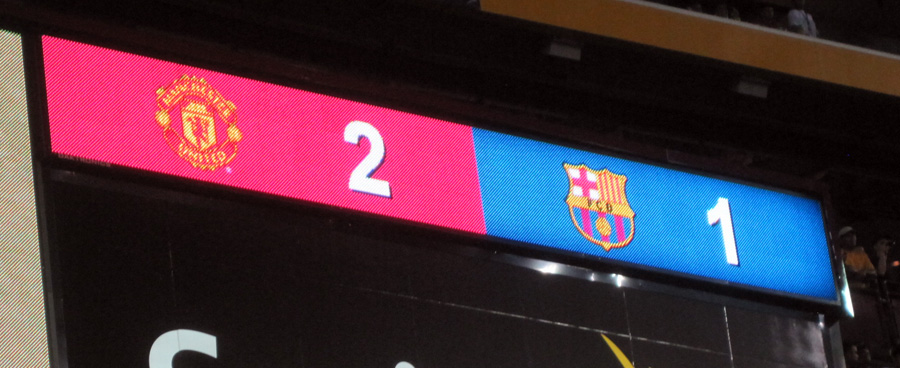
\includegraphics[width=3in]{Gr10-Probability-images/5996076302_412ec8d8d0_o.jpg}
 \\
  \begin{caption*}{(Picture by apasciuto on Flickr.com)}\end{caption*}
 \end{center}
\end{figure}

\Definition{Sample space}{The sample space of an experiment is
  the set of all possible outcomes of that experiment. The sample
  space is denoted with the symbol \(S\) and the size of the sample
  space (the total number of possible outcomes) is denoted with
  \(n(S)\).}

Even though we are usually interested in the outcome of an experiment,
we also need to know what the other outcomes could have been. Let's
have a look at the sample spaces of each of our three experiments.

\paragraph{Experiment 1} Since a coin can land in one of only two ways
(we will ignore the possibility that the coin lands on its edge), the
sample space is the set \(S=\{\mbox{H}; \mbox{T}\}\). The size of the sample space of the coin toss
is \(n(S)=2\):

\begin{figure}[H]
  \begin{center}
  \begin{tikzpicture}
    \begin{scope}[xshift=-1.5cm]
      \coinheads
    \end{scope}
    \begin{scope}[xshift=+1.5cm]
      \cointails
    \end{scope}
    \draw (-3, -1.5) rectangle (3, 1.5) node[anchor=south east] {$S$};
  \end{tikzpicture}
  \end{center}
%   \caption{Sample space of a coin toss.}
\end{figure} 

\paragraph{Experiment 2} Each of the dice can land on a number from $1$
to $6$. In this experiment the sample space of all possible outcomes is
every possible combination of the $6$ numbers on the first die with the
$6$ numbers on the second die. This gives a total of \(n(S) = 6 \times 6
= 36\) possible outcomes. The figure below shows all of the outcomes
in the sample space of rolling two dice:

\begin{figure}[H]
\begin{center}
\begin{tikzpicture}
  \begin{scope}[scale=0.5]
  \foreach \x in {1, ..., 6} {
    \foreach \y in {1, ..., 6} {
      \pgfmathparse{15*rand} \let\rot\pgfmathresult
      \makediesmall{\x}{shift={(4cm*\x-0.66cm,-2cm*\y)},rotate=\rot}
      \pgfmathparse{15*rand} \let\rot\pgfmathresult
      \makediesmall{\y}{shift={(4cm*\x+0.66cm,-2cm*\y)},rotate=\rot}
    }
  }
  \draw[thick] (2.5cm-0.66cm, -0.5cm) rectangle (25.5cm+0.66cm, -13.5cm);
  \draw (25.5cm+0.66cm, -0.5cm) node[anchor=south east] {$S$};
  \end{scope}
\end{tikzpicture}
\end{center}
%   \caption{Sample space of rolling two dice.}
\end{figure} 

\paragraph{Experiment 3} Each soccer team can get an integer score
from $0$ upwards. Usually we don't expect a score to go much higher than
$5$ goals, but there is no reason why this cannot happen. So the sample
space of this experiment consists of all possible combinations of two
non-negative integers. The figure below shows all of the
possibilities. Since we do not limit the score of a team, this sample
space is infinitely large:

\begin{figure}[H]
\begin{center}
  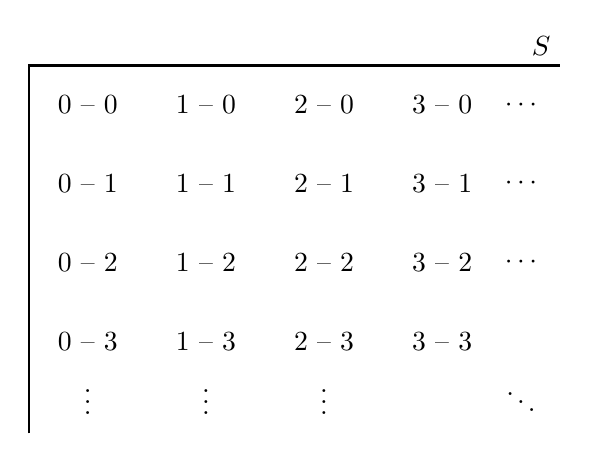
\begin{tikzpicture}
    \foreach \x in {0, ..., 3} {
      \foreach \y in {0, ..., 3} {
        \draw (\x*1.5cm,-\y) node {\x\ --\ \y};
      }
    }
    \foreach \x in {0, ..., 2} {
      \draw (\x*1.5cm,-3.67cm) node {$\vdots$};
    }
    \foreach \y in {0, ..., 2} {
      \draw (5.5cm,-\y) node {$\cdots$};
    }
    \draw (5.5cm,-3.67cm) node {$\ddots$};

    \draw[thick] (-0.75cm, -4.17cm) -- (-0.75, 0.5cm) -- (6cm, 0.5cm);
    \draw (6cm, 0.5cm) node[anchor=south east] {$S$};
  \end{tikzpicture}
\end{center}
%   \caption{Sample space of the final score of a soccer match.}
\end{figure}

\Definition{Event}{An event is a specific set of outcomes of an
  experiment that you are interested in. An event is denoted with the
  letter \(E\) and the number of outcomes in the event with \(n(E)\).}

\paragraph{Experiment 1} Let's say that we would like the coin to land
heads up. Here the event contains a single outcome:
\(E=\{\mbox{H}\}\), \(n(E)=1\).

\paragraph{Experiment 2} Let's say that we are interested in the sum
of the dice being $8$. In this case the event set is
$E=\{($\raisebox{-2pt}{\begin{tikzpicture}
  \begin{scope}[scale=0.333]
    \makediegeneral{2}{xshift=-0.7cm}{0.175cm*0.333}
    \makediegeneral{6}{xshift=+0.7cm}{0.175cm*0.333}
  \end{scope}
\end{tikzpicture}}$);($\raisebox{-2pt}{\begin{tikzpicture}
  \begin{scope}[scale=0.333]
    \makediegeneral{3}{xshift=-0.7cm}{0.175cm*0.333}
    \makediegeneral{5}{xshift=+0.7cm}{0.175cm*0.333}
  \end{scope}
\end{tikzpicture}}$);($\raisebox{-2pt}{\begin{tikzpicture}
  \begin{scope}[scale=0.333]
    \makediegeneral{4}{xshift=-0.7cm}{0.175cm*0.333}
    \makediegeneral{4}{xshift=+0.7cm}{0.175cm*0.333}
  \end{scope}
\end{tikzpicture}}$);($\raisebox{-2pt}{\begin{tikzpicture}
  \begin{scope}[scale=0.333]
    \makediegeneral{5}{xshift=-0.7cm}{0.175cm*0.333}
    \makediegeneral{3}{xshift=+0.7cm}{0.175cm*0.333}
  \end{scope}
\end{tikzpicture}}$);($\raisebox{-2pt}{\begin{tikzpicture}
  \begin{scope}[scale=0.333]
    \makediegeneral{6}{xshift=-0.7cm}{0.175cm*0.333}
    \makediegeneral{2}{xshift=+0.7cm}{0.175cm*0.333}
  \end{scope}
\end{tikzpicture}}$)\}$
since it contains all of the possible ways to get $8$ dots with $2$ dice.
The size of the event set is \(n(E)=5\).

%We can also represent this visually by drawing a line around the
%outcomes in which we are interested.
%FIGURE: sample space with closed curve around event set

\paragraph{Experiment 3} We would like to know whether the first team
will win. For this event to happen the first score must be greater
than the second.
\[E=\{(1;0);(2;0);(2;1);(3;0);(3;1);(3;2);\ldots\}\]
This event set is infinitely large.

%FIGURE: sample space with open curve around event set

\section{Theoretical probability}
\Definition{Probability}{A probability is a real number between
  $0$ and $1$ that describes how likely it is that an event will occur.}
\begin{itemize}
\item A probability of $0$ means that an event will never occur.
\item A probability of $1$ means that an event will always occur.
\item A probability of $0,5$ means that an event will occur half the
  time, or $1$ time out of every $2$.
\end{itemize}

When all of the possible outcomes of an experiment have an equal
chance of occurring, we can compute the exact theoretical probability
of an event. The probability of an event is the ratio between the
number of outcomes in the event set and the number of possible
outcomes in the sample space.
\[P(E) = \frac{n(E)}{n(S)}\]

\mindsetvid{Calculating probabilities}{VMbzp}

\begin{wex}{Theoretical probabilities}
{What is the theoretical probability of each of the events in the
  first two of our three experiments?}
{
  \westep{Write down the size of the sample space}

  \begin{itemize}
  \item[] Experiment 1 (coin): $n(S) = 2$
  \item[] Experiment 2 (dice): $n(S) = 36$
  \end{itemize}
  
  \westep{Write down the size of the event set}

  \begin{itemize}
  \item[] Experiment 1: $n(E) = 1$
  \item[] Experiment 2: $n(E) = 5$
  \end{itemize}

  \westep{Compute the theoretical probability}

  \begin{itemize}
  \item[] Experiment 1: $P(E) = \dfrac{n(E)}{n(S)} = \dfrac{1}{2} = 0,5$
  \item[] Experiment 2: $P(E) = \dfrac{n(E)}{n(S)} = \dfrac{5}{36} = 0,13\dot{8}$
  \end{itemize}
}
\end{wex}

Note that we do not consider the theoretical probability of the third
experiment. The third experiment is different from the first two in an
important way, namely that all possible outcomes (all final scores)
are not equally likely. For example, we know that a soccer score of
$1$--$1$ is quite common, while a score of $11$--$15$ is very, very
rare. Because all outcomes are not equally likely, we cannot use the
ratio between \(n(E)\) and \(n(S)\) to compute the theoretical
probability of a team winning. 

% \IFact{The record for the total number of goals scored by both teams in the FIFA World Cup is $12$. This
% was achieved in $1954$ in the match between Austria and Switzerland, where the final score was $7$--$5$.}

\begin{exercises}{}
{
  \begin{enumerate}[itemsep=5pt, label=\textbf{\arabic*}. ]
  \item 
A bag contains $6$ red, $3$ blue, $2$ green and $1$ white
    balls. A ball is picked at random. Determine the probability that it
    is:
    \begin{enumerate}[noitemsep, label=\textbf{(\alph*)} ]
    \item red
    \item blue or white
    \item not green
    \item not green or red
    \end{enumerate}
  \item 
A playing card is selected randomly from a pack of $52$
    cards. Determine the probability that it is:
    \begin{enumerate}[noitemsep, label=\textbf{(\alph*)} ]
% \setcounter{enumi}{4}
    \item the $2$ of hearts
    \item a red card
    \item a picture card
    \item an ace
    \item a number less than $4$
    \end{enumerate}
\item Even numbers from $2$ to $100$ are written on cards. 
  What is
    the probability of selecting a multiple of $5$, if a card is drawn
    at random?

\end{enumerate}
\practiceinfo

\begin{tabular}{cccccc}
    (1.) 00id& (2.) 00ie& (3.) 00if\\
  \end{tabular}
}
\end{exercises}

\section{Relative frequency}

\Definition{Relative frequency}{The relative frequency of an event is
  defined as the number of times that the event occurs during
  experimental trials, divided by the total number of trials
  conducted.}

The relative frequency is not a theoretical quantity, but an
experimental one. We have to repeat an experiment a number of times
and count how many times the outcome of the trial is in the event
set. Because it is experimental, it is possible to get a different
relative frequency every time that we repeat an experiment.\par
\mindsetvid{Relative frequency}{VMbzy}
\begin{wex}{Relative frequency and theoretical probability}
{We toss a coin $30$ times and observe the outcomes. The results of
  the trials are shown in the table below.
%  \vspace*{\baselineskip}

  \begin{center}
    \begin{tabular}{lc@{\hspace{0.25cm}}c@{\hspace{0.25cm}}c@{\hspace{0.25cm}}c@{\hspace{0.25cm}}c@{\hspace{0.25cm}}c@{\hspace{0.25cm}}c@{\hspace{0.25cm}}c@{\hspace{0.25cm}}c@{\hspace{0.25cm}}c}
      \toprule
      trial   &  $1$ &  $2$ &  $3$ &  $4$ &  $5$ &  $6$ &  $7$ &  $8$ &  $9$ & $10$ \\
      outcome &  H &  T &  T &  T &  H &  T &  H &  H &  H &  T \\
      \midrule
      trial   & $11$ & $12$ & $13$ & $14$ & $15$ & $16$ & $17$ & $18$ & $19$ & $20$ \\
      outcome &  H &  T &  T &  H &  T &  T &  T &  H &  T &  T \\
      \midrule
      trial   & $21$ & $22$ & $23$ & $24$ & $25$ & $26$ & $27$ & $28$ & $29$ & $30$ \\
      outcome &  H &  H &  H &  T &  H &  T &  H &  T &  T &  T \\
      \bottomrule
    \end{tabular}
  \end{center}
  \vspace{8pt}\\

  What is the relative frequency of observing heads after each trial
  and how does it compare to the theoretical probability of observing
  heads?
}{
  \westep{Count the number of positive outcomes}

  A positive outcome is when the outcome is in our event set. The
  table below shows a running count (after each trial $t$) of the
  number of positive outcomes $p$ we have observed. For example, after
  $t=20$ trials we have observed heads $8$ times and tails $12$ times and
  so the positive outcome count is $p=8$.

  \begin{center}
    \begin{tabular}{cc@{\hspace{0.25cm}}c@{\hspace{0.25cm}}c@{\hspace{0.25cm}}c@{\hspace{0.25cm}}c@{\hspace{0.25cm}}c@{\hspace{0.25cm}}c@{\hspace{0.25cm}}c@{\hspace{0.25cm}}c@{\hspace{0.25cm}}c}
      \toprule
      $t$ &  $1$ &  $2$ &  $3$ &  $4$ &  $5$ &  $6$ &  $7$ &  $8$ &  $9$ & $10$ \\
      $p$ &  $1$ &  $1$ &  $1$ &  $1$ &  $2$ &  $2$ &  $3$ &  $4$ &  $5$ &  $5$ \\
      \midrule
      $t$ & $11$ & $12$ & $13$ & $14$ & $15$ & $16$ & $17$ & $18$ & $19$ & $20$ \\
      $p$ &  $6$ &  $6$ &  $6$ &  $7$ &  $7$ &  $7$ &  $7$ &  $8$ &  $8$ &  $8$ \\
      \midrule
      $t$ & $21$ & $22$ & $23$ & $24$ & $25$ & $26$ & $27$ & $28$ & $29$ & $30$ \\
      $p$ &  $9$ & $10$ & $11$ & $11$ & $12$ & $12$ & $13$ & $13$ & $13$ & $13$ \\
      \bottomrule
    \end{tabular}
  \end{center}
  \vspace{8pt}\\

  \westep{Compute the relative frequency}

  Since the relative frequency is defined as the ratio between the
  number of positive trials and the total number of trials,
  \[f=\frac{p}{t}\]
  The relative frequency of observing heads, $f$, after having
  completed $t$ coin tosses is:

  \begin{center}
    \begin{tabular}{cc@{\hspace{0.25cm}}c@{\hspace{0.25cm}}c@{\hspace{0.25cm}}c@{\hspace{0.25cm}}c@{\hspace{0.25cm}}c@{\hspace{0.25cm}}c@{\hspace{0.25cm}}c@{\hspace{0.25cm}}c@{\hspace{0.25cm}}c}
      \toprule
      $t$ &  $1$ &  $2$ &  $3$ &  $4$ &  $5$ &  $6$ &  $7$ &  $8$ &  $9$ & $10$ \\
      $f$ & $1,00$ & $0,50$ & $0,33$ & $0,25$ & $0,40$ & $0,33$ & $0,43$ & $0,50$ & $0,56$ & $0,50$ \\
      \midrule
      $t$ & $11$ & $12$ & $13$ & $14$ & $15$ & $16$ & $17$ & $18$ & $19$ & $20$ \\
      $f$ & $0,55$ & $0,50$ & $0,46$ & $0,50$ & $0,47$ & $0,44$ & $0,41$ & $0,44$ & $0,42$ & $0,40$ \\
      \midrule
      $t$ & $21$ & $22$ & $23$ & $24$ & $25$ & $26$ & $27$ & $28$ & $29$ & $30$ \\
      $f$ & $0,43$ & $0,45$ & $0,48$ & $0,46$ & $0,48$ & $0,46$ & $0,48$ & $0,46$ & $0,45$ & $0,43$ \\
      \bottomrule
    \end{tabular}
  \end{center}
  \vspace{8pt}\\
  
From the last entry in this table we can now easily read the relative
frequency after $30$ trials, namely $13/30 = 0,4\dot{3}$. The relative
frequency is close to the theoretical probability of $0,5$. In general,
the relative frequency of an event tends to get closer to the theoretical
probability of the event as we perform more trials.\\
\\
A much better way to summarise the table of relative frequencies is in
a graph: 

\begin{figure}[H]
  \begin{center}
    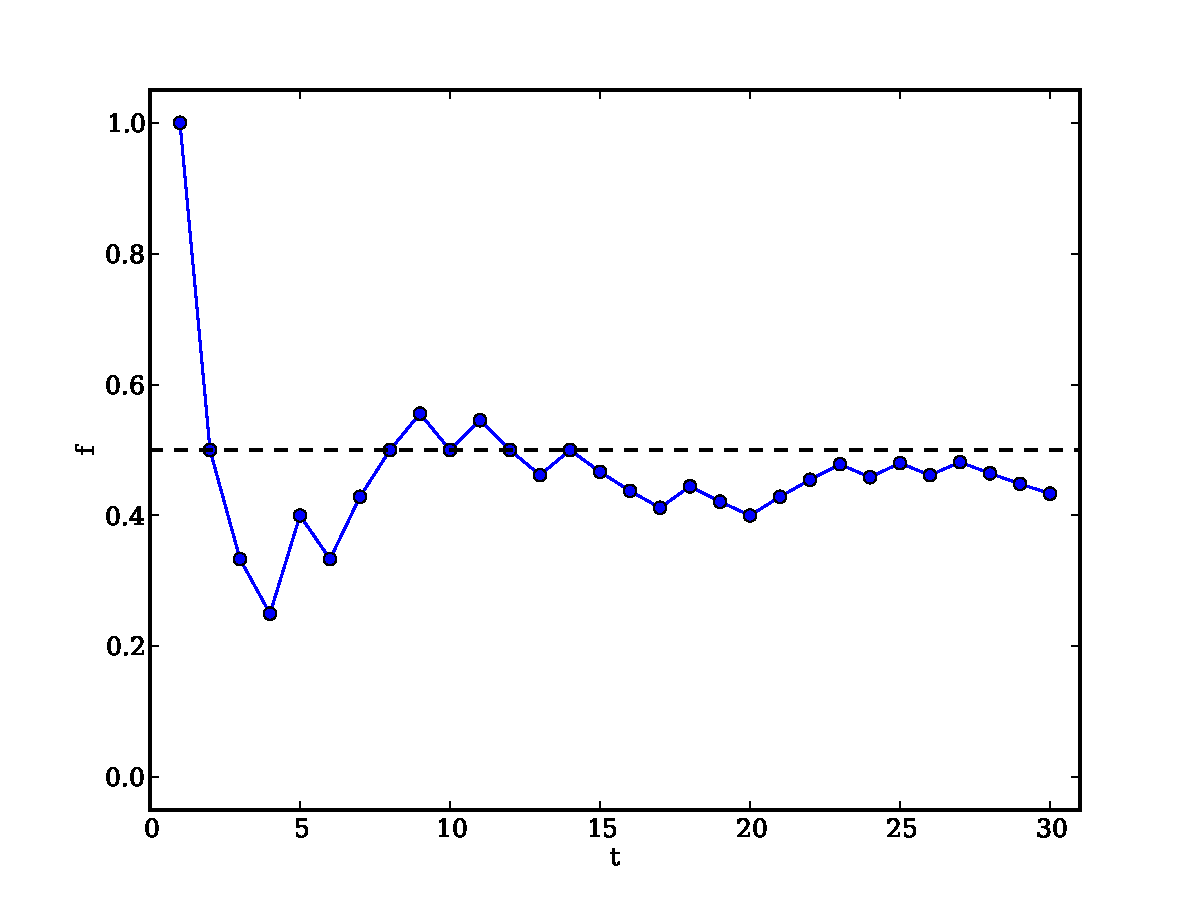
\includegraphics[width=0.75\textwidth]{Gr10-Probability-images/coin_toss_trials.pdf}
  \end{center}
%   \caption{Plot of the relative frequency of observing heads, $f$,
%     after having completed $t$ coin tosses.}
\end{figure}

\noindent The graph above is the plot of the relative frequency of observing heads, $f$,
after having completed $t$ coin tosses. It was generated from the table of numbers above
by plotting the number of trials that have been completed, $t$, on the
$x$-axis and the relative frequency, $f$, on the $y$-axis. In the
beginning (after a small number of trials) the relative frequency
fluctuates a lot around the theoretical probability at $0,5$, which is
shown with a dashed line. As the number of trials increases, the
relative frequency fluctuates less and gets closer to the theoretical
probability. 
}
\end{wex}

%\paragraph{Experiment 2} We roll the two dice $100$ times and observe
%whether the sum of the dice equals $8$. It turns out that our event
%occurs $15$ times during the experiment. From this we can calculate the
%relative frequency as
%\[\frac{15}{100}=0,15\]
%This is close to the theoretical probability, which we compute earlier
%as $0,13\dot{8}$.

\begin{wex}{Relative frequency and theoretical probability}
{While watching $10$ soccer games where Team 1 plays against Team 2, we
  record the following final scores:
    \begin{center}
      \begin{tabular}{lcccccccccc}
        \toprule
        Trial  & $1$ & $2$ & $3$ & $4$ & $5$ & $6$ & $7$ & $8$ & $9$ & $10$ \\
        \midrule
        Team 1 & $2$ & $0$ & $1$ & $1$ & $1$ & $1$ & $1$ & $0$ & $5$ & $3$ \\
        Team 2 & $0$ & $2$ & $2$ & $2$ & $2$ & $1$ & $1$ & $0$ & $0$ & $0$ \\
        \bottomrule
      \end{tabular}
    \end{center}

What is the relative frequency of Team 1 winning?
}
{In this experiment, each trial takes the form of Team 1 playing a
  soccer match against Team 2.

  \westep{Count the number of positive outcomes}

  We are interested in the event where Team 1 wins. From the table
  above we see that this happens $3$ times.

  \westep{Compute the relative frequency}

  The total number of trials is $10$. This means that the relative
  frequency of the event is \[\frac{3}{10} = 0,3\]
}
\end{wex}

It is important to understand the difference between the theoretical
probability of an event and the observed relative frequency of the
event in experimental trials. The theoretical probability is a number
that we can compute if we have enough information about the
experiment. If each possible outcome in the sample space is
equally likely, we can count the number of outcomes in the event set
and the number of outcomes in the sample space to compute the
theoretical probability.\par

The relative frequency depends on the sequence of outcomes that we
observe while doing a statistical experiment. The relative frequency
can be different every time we redo the experiment. The more trials we
run during an experiment, the closer the observed relative frequency
of an event will get to the theoretical probability of the event.\par

So why do we need statistical experiments if we have theoretical
probabilities? In some cases, like our soccer experiment, it is
difficult or impossible to compute the theoretical probability of an
event. Since we do not know exactly how likely it is that one soccer
team will score goals against another, we can never compute the
theoretical probability of events in soccer. In such cases we can
still use the relative frequency to estimate the theoretical
probability, by running experiments and counting the number of
positive outcomes.\par

\section{Venn diagrams}
A Venn diagram is a graphical way of representing the relationships
between sets. In each Venn diagram a set is represented by a closed
curve. The region inside the curve represents the elements that
belong to the set, while the region outside the curve represents the
elements that are excluded from the set.\par

Venn diagrams are helpful for thinking about probability since we deal
with different sets. Consider two events, $A$ and $B$, in a sample
space $S$.
%  Figure~\ref{fig:venndiagrams} 
The diagram below shows the possible ways in which the event
sets can overlap, represented using Venn diagrams:\\

\begin{figure}[H]
\begin{center}
\scalebox{1} % Change this value to rescale the drawing.
{
\begin{pspicture}(0,-1.701875)(10.96,1.721875)
\psframe[linewidth=0.04,dimen=outer](3.0,1.298125)(0.0,-1.701875)
\pscircle[linewidth=0.04,dimen=outer](0.78,-0.061875){0.56}
\pscircle[linewidth=0.04,dimen=outer](1.83,-0.371875){0.91}
\usefont{T1}{ptm}{m}{n}
\rput(0.7265625,0.728125){$A$}
\usefont{T1}{ptm}{m}{n}
\rput(1.8471875,0.768125){$B$}
\usefont{T1}{ptm}{m}{n}
\rput(2.8192186,1.528125){$S$}
\psframe[linewidth=0.04,dimen=outer](6.98,1.318125)(3.98,-1.681875)
\pscircle[linewidth=0.04,dimen=outer](4.7,-0.961875){0.56}
\pscircle[linewidth=0.04,dimen=outer](6.02,-0.001875){0.8}
\usefont{T1}{ptm}{m}{n}
\rput(4.7065625,-0.191875){$A$}
\usefont{T1}{ptm}{m}{n}
\rput(6.0071874,1.008125){$B$}
\usefont{T1}{ptm}{m}{n}
\rput(6.7992187,1.548125){$S$}
\psframe[linewidth=0.04,dimen=outer](10.96,1.318125)(7.96,-1.681875)
\pscircle[linewidth=0.04,dimen=outer](9.38,0.078125){0.56}
\pscircle[linewidth=0.04,dimen=outer](9.47,-0.271875){1.13}
\usefont{T1}{ptm}{m}{n}
\rput(10.266562,0.828125){$A$}
\usefont{T1}{ptm}{m}{n}
\rput(9.447187,-0.811875){$B$}
\usefont{T1}{ptm}{m}{n}
\rput(10.779219,1.548125){$S$}
\end{pspicture} 
}
%   \caption{Venn diagrams with different configurations of two events,
%     $A$ and $B$, in a sample space, $S$.}
\end{center}
\label{fig:venndiagrams}
\end{figure}\\

The sets are represented using a rectangle for $S$ and circles for
each of $A$ and $B$.  In the first diagram the two events overlap
partially. In the second diagram the two events do not overlap at
all. In the third diagram one event is fully contained in the other.
Note that events will always appear inside the sample space since the
sample space contains all possible outcomes of the experiment.
% \vspace{-1cm}
\par
\mindsetvid{{V}enn diagrams and probabilities}{VMcbf}
\begin{wex}{Venn diagrams}
{\wexlabel{wex:dice_venn}%
Represent the sample space of two rolled dice and the following two events using a Venn diagram:
  \begin{itemize}
  \item[] Event $A$: the sum of the dice equals $8$
  \item[] Event $B$: at least one of the dice shows\ \raisebox{-2pt}{
      \begin{tikzpicture}
        \begin{scope}[scale=0.333]
          \makediegeneral{2}{}{0.175cm*0.333}
        \end{scope}
      \end{tikzpicture}
    }
  \end{itemize}
}{
\begin{center}
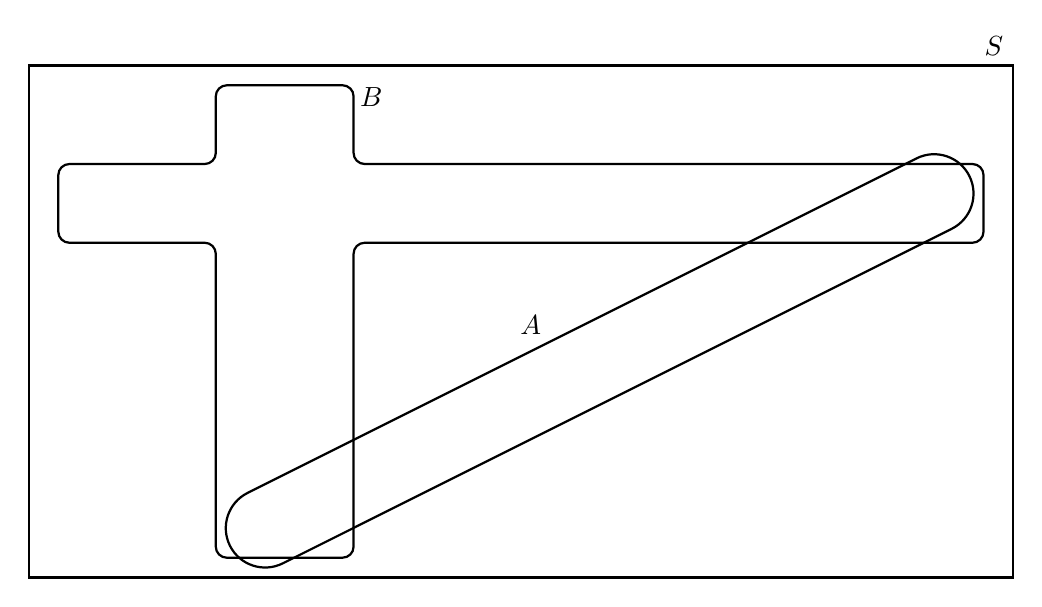
\begin{tikzpicture}
  \begin{scope}[scale=0.5]
    \begin{scope}[draw=gray,fill=gray]
      \foreach \x in {1, ..., 6} {
        \foreach \y in {1, ..., 6} {
          \pgfmathparse{15*rand} \let\rot\pgfmathresult
          \makediesmall{\x}{shift={(4cm*\x-0.66cm,-2cm*\y)},rotate=\rot}
          \pgfmathparse{15*rand} \let\rot\pgfmathresult
          \makediesmall{\y}{shift={(4cm*\x+0.66cm,-2cm*\y)},rotate=\rot}
        }
      }
    \end{scope}
    \draw[thick] (1.5cm, -0.5cm) rectangle (26.5cm, -13.5cm);
    \draw (26.5cm, -0.5cm) node[anchor=south east] {$S$};
    \draw[thick,rounded corners]
      (6.25cm, -1cm) -- (6.25cm, -3cm) -- (2.25cm, -3cm) -- (2.25cm, -5cm) --
      (6.25cm, -5cm) -- (6.25cm, -13cm) -- (9.75cm, -13cm) -- (9.75cm, -5cm) --
      (25.75cm, -5cm) -- (25.75cm, -3cm) -- (9.75cm, -3cm) -- (9.75cm, -1cm) -- cycle;
    \draw (10.2cm, -1.3cm) node {$B$};
    \begin{scope}[xshift=16cm,yshift=-8cm,rotate=26.57]
      \def\d{9.5cm}
      \def\r{1cm}
      \draw[thick]
        (+\d, +\r) -- (-\d, +\r) arc (90:270:\r) -- 
        (+\d, -\r) arc (-90:90:\r) -- cycle;
    \end{scope}
    \draw (14.25cm, -7.1cm) node {$A$};
  \end{scope}
\end{tikzpicture}
\end{center}
}
\end{wex}

\begin{wex}{Venn diagrams}
{Consider the set of diamonds removed from a deck of cards. A random card is selected from the set of diamonds.
\begin{itemize}
 \item Write down the sample space, $S$, for the experiment.
\item What is the value of $n(S)$?
\item Consider the following two events:
\begin{itemize}
\item $P$: An even diamond is chosen
\item $R$: A royal diamond is chosen
\end{itemize}
Represent sample space $S$ and events $P$ and $R$ using a Venn diagram.
\end{itemize}
}
{
\westep{Write down the sample space $S$}
\begin{align*}
S=\{A;~2;~3;~4;~5;~6;~7;~8;~9;~10;~J;~Q;~K\}
\end{align*}
\westep{Write down the value of $n(S)$}
\begin{align*}
 n(S) = 13
\end{align*}
\westep{Draw the Venn diagram}
\begin{center}
\scalebox{1} % Change this value to rescale the drawing.
{
\begin{pspicture}(0,-2.2)(4.5590625,2.2)
\pscircle[linewidth=0.04,dimen=outer](2.2,0.0){2.2}
\pscircle[linewidth=0.04,dimen=outer](1.45,-0.03){1.29}
\pscircle[linewidth=0.04,dimen=outer](2.54,0.76){0.9}
% \usefont{T1}{ptm}{m}{n}
\rput(3.7,1.9){$S$}
% \usefont{T1}{ptm}{m}{n}
\rput(2.9945312,0.83){$J$}
% \usefont{T1}{ptm}{m}{n}
\rput(2.4745312,1.29){$K$}
% \usefont{T1}{ptm}{m}{n}
\rput(2.1745312,0.53){$Q$}
% \usefont{T1}{ptm}{m}{n}
\rput(1.1445312,0.71){$2$}
% \usefont{T1}{ptm}{m}{n}
\rput(0.70453125,0.05){$4$}
% \usefont{T1}{ptm}{m}{n}
\rput(1.5645312,0.07){$6$}
% \usefont{T1}{ptm}{m}{n}
\rput(1.1245313,-0.55){$8$}
% \usefont{T1}{ptm}{m}{n}
\rput(2.0945313,-0.51){$10$}
% \usefont{T1}{ptm}{m}{n}
\rput(3.0845313,-0.77){$3$}
% \usefont{T1}{ptm}{m}{n}
\rput(3.8845313,-0.49){$5$}
% \usefont{T1}{ptm}{m}{n}
\rput(2.5445313,-1.45){$7$}
% \usefont{T1}{ptm}{m}{n}
\rput(3.4245312,-1.25){$9$}
% \usefont{T1}{ptm}{m}{n}
\rput(3.7745314,0.23){$A$}
% \usefont{T1}{ptm}{m}{n}
\rput(1.0145313,1.37){$P$}
% \usefont{T1}{ptm}{m}{n}
\rput(2.5045311,1.83){$R$}
\end{pspicture} 
}
\end{center}
}
\end{wex}

\begin{exercises}{}{
%  \begin{enumerate}[itemsep=5pt, label=\textbf{\arabic*}. ]
  \item Let $S$ denote the set of whole numbers from $1$ to $16$, $X$
    denote the set of even numbers from $1$ to $16$ and $Y$ denote the
    set of prime numbers from $1$ to $16$. Draw a Venn diagram depicting $S$, $X$ and $Y$.
%     \item Find $n\left(S\right)$, $n\left(X\right)$, $n\left(Y\right)$,
%       $n\left(X\cup Y\right)$, $n\left(X\cap Y\right)$.
%  \end{enumerate}
\item
  There are $79$ Grade $10$ learners at school. All of these
    take some combination of Maths, Geography and History. The number who take
    Geography is $41$, those who take History is $36$, and $30$ take
    Maths. The number who take Maths and History is $16$; the number
    who take Geography and History is $6$, and there are $8$ who take
    Maths only and $16$ who take History only.
    \begin{enumerate}[noitemsep, label=\textbf{(\alph*)} ]

    \item Draw a Venn diagram to illustrate all this information.
    \item How many learners take Maths and Geography but not History?
    \item How many learners take Geography only?
    \item How many learners take all three subjects?
    \end{enumerate}
 \item Pieces of paper labelled with the numbers $1$ to $12$ are
    placed in a box and the box is shaken. One piece of paper is taken
    out and then replaced.
    \begin{enumerate}[noitemsep, label=\textbf{(\alph*)} ]

    \item What is the sample space, $S$?
    \item Write down the set $A$, representing the event of taking a
      piece of paper labelled with a factor of $12$.
    \item Write down the set $B$, representing the event of taking a
      piece of paper labelled with a prime number.
    \item Represent $A$, $B$ and $S$ by means of a Venn diagram.
    \item Find
      \begin{enumerate}[noitemsep, label=\textbf{\roman*.} ]
      \item $n\left(S\right)$
      \item $n\left(A\right)$
      \item $n\left(B\right)$
%       \item $n\left(A\cap B\right)$
%       \item $n\left(A\cup B\right)$
      \end{enumerate}
%     \item Is $n\left(A\cup B\right)=n\left(A\right)+n\left(B\right)-n\left(A\cap B\right)$?
    \end{enumerate}
  \item In a school survey 80 learners were questioned to find whether newspaper X or newspaper Y is the popular choice of newspaper for school-goers.  The survey revealed that 45 learners read newspaper X, 30 learners read newspaper Y and 10 learners read neither.\\
  Use a Venn diagram to determine how many learners read:
    \begin{enumerate}[noitemsep, label=\textbf{(\alph*)} ]
    \item Newspaper X on?
    \item Write down the set $A$, representing the event of taking a
      piece of paper labelled with a factor of $12$.
    \item Write down the set $B$, representing the event of taking a
      piece of paper labelled with a prime number.
  \end{enumerate}
\practiceinfo

\begin{tabular}{cccccc}
    (1.) 00ig& (2.) 00ih& (3.) 00ii\\
  \end{tabular}
}
\end{exercises}

\section{Union and intersection}
\Definition{Union}{The union of two sets is a new set that contains
  all of the elements that are in at least one of the two sets. The
  union is written as $A \cup B$.}

\Definition{Intersection}{The intersection of two sets is a new set
  that contains all of the elements that are in both sets. The
  intersection is written as $A \cap B$.}

The figure below shows the union and intersection for different
configurations of two events in a sample space, using Venn diagrams.

\begin{figure}[H]
  \begin{center}
  \begin{tabular}{ccc}
    \begin{tikzpicture}
      \begin{scope}[scale=3]
        \draw \samplespace; \labelsamplespace;
        \draw \circlepartiala; \labelpartiala;
        \draw \circlepartialb; \labelpartialb;
      \end{scope}
    \end{tikzpicture}
    &
    \begin{tikzpicture}
      \begin{scope}[scale=3]
        \draw \samplespace; \labelsamplespace;
        \draw \circleseparatea; \labelseparatea;
        \draw \circleseparateb; \labelseparateb;
      \end{scope}
    \end{tikzpicture}
    &
    \begin{tikzpicture}
      \begin{scope}[scale=3]
        \draw \samplespace; \labelsamplespace;
        \draw \circlefulla; \labelfulla;
        \draw \circlefullb; \labelfullb;
      \end{scope}
    \end{tikzpicture}
    \\
    \begin{tikzpicture}
      \begin{scope}[scale=3]
        \draw \samplespace; \labelsamplespace;
        \draw[fill=lightgray] (0.31369, 0.31041) arc (-162.62:130.73:0.3cm) arc (39.54:288.57:0.2cm);
        \draw[dotted] (0.31369, 0.31041) arc (197.38:130.73:0.3cm) arc (39.54:-71.43:0.2cm);
        \draw (0.4,0.7) node[anchor=south] {$A \cup B$};
      \end{scope}
    \end{tikzpicture}
    &
    \begin{tikzpicture}
      \begin{scope}[scale=3]
        \draw \samplespace; \labelsamplespace;
        \draw[fill=lightgray] \circleseparatea;
        \draw[fill=lightgray] \circleseparateb;
        \draw (0.3,0.2) node[anchor=west] {$A \cup B$};
      \end{scope}
    \end{tikzpicture}
    &
    \begin{tikzpicture}
      \begin{scope}[scale=3]
        \draw \samplespace; \labelsamplespace;
        \draw[fill=lightgray] \circlefulla;
        \draw[dotted] \circlefullb;
        \draw (0.5,0.83) node[anchor=south] {$A \cup B$};
      \end{scope}
    \end{tikzpicture}
    \\
    \begin{tikzpicture}
      \begin{scope}[scale=3]
        \draw \samplespace; \labelsamplespace;
        \draw[dotted] (0.31369, 0.31041) arc (-162.62:130.73:0.3cm) arc (39.54:288.57:0.2cm);
        \draw[fill=lightgray] (0.31369, 0.31041) arc (197.38:130.73:0.3cm) arc (39.54:-71.43:0.2cm);
        \draw (0.4,0.65) node[anchor=south] {$A \cap B$};
      \end{scope}
    \end{tikzpicture}
    &
    \begin{tikzpicture}
      \begin{scope}[scale=3]
        \draw \samplespace; \labelsamplespace;
        \draw[dotted] \circleseparatea;
        \draw[dotted] \circleseparateb;
      \end{scope}
    \end{tikzpicture}
    &
    \begin{tikzpicture}
      \begin{scope}[scale=3]
        \draw \samplespace; \labelsamplespace;
        \draw[dotted] \circlefulla;
        \draw[fill=lightgray] \circlefullb;
        \draw (0.5,0.75) node[anchor=south] {$A \cap B$};
      \end{scope}
    \end{tikzpicture}
    \\
  \end{tabular}
\end{center}

  \begin{caption*}{The unions and intersections of different events. Note that
    in the middle column the intersection, $A \cap B$, is empty since
    the two sets do not overlap. In the final column the union,
    $A \cup B$, is equal to $A$ and the intersection, $A \cap B$, is
    equal to $B$ since $B$ is fully contained in $A$.}\end{caption*}
  \label{fig:venn_union_intersection}
\end{figure}
\par
\mindsetvid{Inclusive and exclusive events}{VMcci}
\section{Probability identities}
\begin{equation*}
 P(S)=1
\end{equation*}


By definition, the sample space contains all possible outcomes of an
experiment. So we know that the probability of observing an outcome
from the sample space is $1$.

\begin{equation*}
 P(A \cup B) = P(A) + P(B) - P(A \cap B)
\end{equation*}


We will prove this identity using the Venn diagrams given above.

% \ref{fig:venn_union_intersection}
For each of the $4$ terms in the
union and intersection identity, we can draw the Venn diagram and then
add and subtract the different diagrams. The area of a region
represents its probability.

We will do this for the first column of the Venn diagram figure given previously% \ref{fig:venn_union_intersection}
. You should also try it for the
other columns.

\begin{center}
\begin{tabular}{m{0.5cm}m{1.5cm}m{0.5cm}m{0.3cm}@{\hspace{0.1cm}}m{1.5cm}m{0.5cm}m{1.5cm}@{\hspace{0.1cm}}m{0.3cm}}
   & $P(A)$ & $+$ && $P(B)$ & $-$ & $P(A \cap B)$ \\[4pt]
 $=$ & \begin{tikzpicture}
   \begin{scope}[scale=1.5]
     \draw \samplespace;
     \draw[fill=lightgray] \circlepartiala;
   \end{scope}
\end{tikzpicture} & $+$ & $\Bigg($ & \begin{tikzpicture}
   \begin{scope}[scale=1.5]
     \draw \samplespace;
     \draw[fill=lightgray] \circlepartialb;
   \end{scope}
\end{tikzpicture} & $-$ & \begin{tikzpicture}
   \begin{scope}[scale=1.5]
     \draw \samplespace;
     \draw[fill=lightgray] (0.31369, 0.31041) 00ij(197.38:130.73:0.3cm) 00mk(39.54:-71.43:0.2cm);
   \end{scope}
\end{tikzpicture} & $\Bigg)$ \\[4pt]
$ =$ & \begin{tikzpicture}
   \begin{scope}[scale=1.5]
     \draw \samplespace;
     \draw[fill=lightgray] \circlepartiala;
   \end{scope}
\end{tikzpicture} & $+$ && \begin{tikzpicture}
   \begin{scope}[scale=1.5]
     \draw \samplespace;
     \draw[fill=lightgray] (0.31369, 0.31041) 00ik(-162.62:130.73:0.3cm) 00mm(39.54:-71.43:0.2cm);
   \end{scope}
\end{tikzpicture} \\[4pt]
 $=$ & \begin{tikzpicture}
      \begin{scope}[scale=1.5]
        \draw \samplespace;
        \draw[fill=lightgray] (0.31369, 0.31041) 00im(-162.62:130.73:0.3cm) 00mn(39.54:288.57:0.2cm);
      \end{scope}
\end{tikzpicture} \\[4pt]
$ =$ & $P(A \cup B)$
\end{tabular}
\end{center}

\begin{wex}{Union and intersection of events}
{Relate the probabilities of events $A$ and $B$ from
  Worked Example \wexref{wex:dice_venn}
  (two rolled dice) and show that they satisfy the identity
  \[P(A \cup B) = P(A) + P(B) - P(A \cap B).\]
}{
  \westep{Write down the probabilities of the two events, their union
    and their intersection}
  
  From the Venn diagram
  Worked Example \wexref{wex:dice_venn},
 we can count the number of outcomes in each
  event. To get the probability of an event, we divide the size of
  the event by the size of the sample space, which is $n(S)=36$.
  \[\begin{array}{r@{$\ =\ $}c@{$\ =\ $}l}
    P(A)        & \dfrac{n(A)}{n(S)}        & \dfrac{5}{36}  \\[8pt]
    P(B)        & \dfrac{n(B)}{n(S)}        & \dfrac{11}{36} \\[8pt]
    P(A \cap B) & \dfrac{n(A \cap B)}{n(S)} & \dfrac{2}{36}  \\[8pt]
    P(A \cup B) & \dfrac{n(A \cup B)}{n(S)} & \dfrac{14}{36}
  \end{array}\]
  % Sorry for the ugly equation: didn't know how to make the alignment
  % work otherwise

  \westep{Write down and check the identity}
  \begin{align*}
    P(A \cup B) &= P(A) + P(B) - P(A \cap B) \\
    \frac{14}{36} &= \dfrac{5}{36} + \frac{11}{36} - \frac{2}{36} \\
    &= \frac{5}{36} + \frac{9}{36} \\
    &= \frac{14}{36} 
  \end{align*}
}
\end{wex}

\section{Mutually exclusive events}
\Definition{Mutually exclusive events}{Two events are called mutually
  exclusive if they cannot occur at the same time. Whenever an outcome
  of an experiment is in the first event it can not also be in the
  second event, and vice versa.}

Another way of saying this is that the two event sets, $A$ and $B$,
cannot have any elements in common, or $P(A \cap B) = \emptyset$
(where $\emptyset$ denotes the empty set).

We have already seen the Venn diagrams of mutually exclusive events in
the middle column of the Venn diagrams provided on page \pageref{fig:venn_union_intersection}.

% Figure \ref{fig:venn_union_intersection}.

\begin{figure}[H]
  \begin{center}
  \begin{tabular}{ccc}
    \begin{tikzpicture}
      \begin{scope}[scale=3]
        \draw \samplespace; \labelsamplespace;
        \draw \circleseparatea; \labelseparatea;
        \draw \circleseparateb; \labelseparateb;
      \end{scope}
    \end{tikzpicture}
    &
    \begin{tikzpicture}
      \begin{scope}[scale=3]
        \draw \samplespace; \labelsamplespace;
        \draw[fill=lightgray] \circleseparatea;
        \draw[fill=lightgray] \circleseparateb;
        \draw (0.3,0.2) node[anchor=west] {$A \cup B$};
      \end{scope}
    \end{tikzpicture}
    &
    \begin{tikzpicture}
      \begin{scope}[scale=3]
        \draw \samplespace; \labelsamplespace;
        \draw[dotted] \circleseparatea;
        \draw[dotted] \circleseparateb;
        \draw (1,1) node[anchor=south east] {$A \cap B$};
      \end{scope}
    \end{tikzpicture}
  \end{tabular}
\end{center}

\end{figure}

From this figure you can see that the intersection has no
elements. You can also see that the probability of the union is the
sum of the probabilities of the events.
\[P(A \cup B) = P(A) + P(B)\]
This relationship is true for mutually
exclusive events only.

\begin{wex}{Mutually exclusive events}
{We roll two dice and are interested in the following two events:
  \begin{itemize}
  \item[] $A:$ The sum of the dice equals $8$
  \item[] $B:$ At least one of the dice shows\ \raisebox{-2pt}{
      \begin{tikzpicture}
        \begin{scope}[scale=0.333]
          \makediegeneral{1}{}{0.175cm*0.333}
        \end{scope}
      \end{tikzpicture}
    }
  \end{itemize}
  Show that the events are mutually exclusive.
}{
  \westep{Draw the sample space and the two events}

%\begin{figure}[h]
\begin{center}
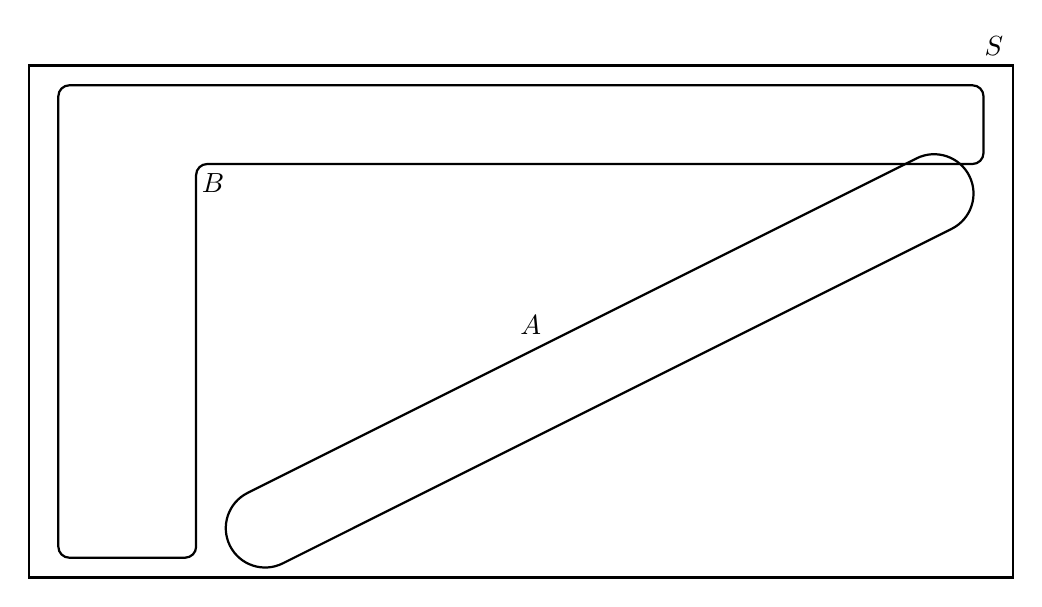
\begin{tikzpicture}
  \begin{scope}[scale=0.5]
    \begin{scope}[draw=gray,fill=gray]
      \foreach \x in {1, ..., 6} {
        \foreach \y in {1, ..., 6} {
          \pgfmathparse{15*rand} \let\rot\pgfmathresult
          \makediesmall{\x}{shift={(4cm*\x-0.66cm,-2cm*\y)},rotate=\rot}
          \pgfmathparse{15*rand} \let\rot\pgfmathresult
          \makediesmall{\y}{shift={(4cm*\x+0.66cm,-2cm*\y)},rotate=\rot}
        }
      }
    \end{scope}
    \draw[thick] (1.5cm, -0.5cm) rectangle (26.5cm, -13.5cm);
    \draw (26.5cm, -0.5cm) node[anchor=south east] {$S$};
    \draw[thick,rounded corners]
      (2.25cm, -1cm) -- (2.25cm, -13cm) -- (5.75cm, -13cm) -- (5.75cm, -3cm) --
      (25.75cm, -3cm) -- (25.75cm, -1cm) -- cycle;
    \draw (5.65cm, -3cm) node[anchor=north west] {$B$};
    \begin{scope}[xshift=16cm,yshift=-8cm,rotate=26.57]
      \def\d{9.5cm}
      \def\r{1cm}
      \draw[thick]
        (+\d, +\r) -- (-\d, +\r) arc (90:270:\r) -- 
        (+\d, -\r) arc (-90:90:\r) -- cycle;
    \end{scope}
    \draw (14.25cm, -7.1cm) node {$A$};
  \end{scope}
\end{tikzpicture}
\end{center}
%\end{figure}

  \westep{Determine the intersection}

  From the above figure we notice that there are no elements in common in
  $A$ and $B$. Therefore the events are mutually exclusive.
}
\end{wex}
%  %manual clearpage to fix broken mdframed for Definition below
\section{Complementary events}

\Definition{Complementary set}{The complement of a set, $A$, is a
  different set that contains all of the elements that are not in
  $A$. We write the complement of $A$ as $A'$, or
  sometimes as ``$\mbox{not}(A)$''.}

For an experiment with sample space $S$ and an event $A$ we can derive
some identities for complementary events. Since every element in $A$ is not in $A'$, we know
  that complementary events are mutually exclusive.
\begin{equation*}
 A \cap A' = \emptyset
\end{equation*}


Since every element in the sample space is either in $A$ or in
  $A'$, the union of complementary events covers the
  sample space.
\begin{equation*}
A \cup A' = S
\end{equation*}
From the previous two identities, we also know that the
  probabilities of complementary events sum to $1$.

\begin{equation*}
P(A) + P(A') = P(A \cup A') = P(S) = 1
\end{equation*}

\mindsetvid{Complementary events}{VMcdl}

% %manual clearpage to fix broken mdframed for Definition below
\begin{wex}{Reasoning with Venn diagrams}
{In a survey $70$ people were questioned about which product they
  use: A or B or both. The report of the survey shows that $25$
  people use product A, $35$ people use product B and $15$ people use
  neither. Use a Venn diagram to work out how many people
  \begin{enumerate}[itemsep=5pt, label=\textbf{\arabic*}. ]
  \item use product A only,
  \item use product B only,
  \item use both product A and product B.
  \end{enumerate}
}{
  \westep{Summarise the sizes of the sample space, the event sets,
    their union and their intersection}
  \begin{itemize}
  \item We are told that $70$ people were questioned, so the size of the
    sample space is $n(S) = 70$.
  \item We are told that $25$ people use product A, so $n(A) = 25$.
  \item We are told that $35$ people use product B, so $n(B) = 35$.
  \item We are told that $15$ people use neither product. This means
    that $70-15=55$ people use at least one of the two products, so
    $n(A \cup B) = 55$.
  \item We are not told how many people use both products, so we have
    to work out the size of the intersection, $A \cap B$, by using the
    identity
    \begin{align*}
      P(A \cup B) &= P(A) + P(B) - P(A \cap B) \\
      \frac{n(A \cup B)}{n(S)} &= \frac{n(A)}{n(S)} + \frac{n(B)}{n(S)} - \frac{n(A \cap B)}{n(S)} \\
      \frac{55}{70} &= \frac{25}{70} + \frac{35}{70} - \frac{n(A \cap B)}{70} \\
      \therefore n(A \cap B) &= 25 + 35 - 55 \\
      &= 5
    \end{align*}
  \end{itemize}

  \westep{Determine whether the events are mutually exclusive}
  Since the intersection of the events, $A \cap B$, is not empty, the
  events are not mutually exclusive. This means that their circles
  should overlap in the Venn diagram.

  \westep{Draw the Venn diagram and fill in the numbers}
    \begin{center}
      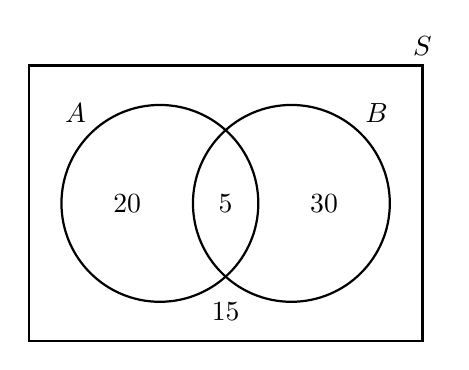
\begin{tikzpicture}
        \begin{scope}[scale=5]
          \draw[thick] (0, 0) rectangle (1cm, 0.7cm);
          \draw (1cm, 0.7cm) node[anchor=south] {$S$};
          \draw[thick] (0.333cm, 0.35cm) circle (0.25cm);
          \draw (0.17, 0.53) node[anchor=south east] {$A$};
          \draw[thick] (0.667cm, 0.35cm) circle (0.25cm);
          \draw (0.83, 0.53) node[anchor=south west] {$B$};
          % Numbers
          \draw (0.5, 0.35) node {$5$};
          \draw (0.25, 0.35) node {$20$};
          \draw (0.75, 0.35) node {$30$};
          \draw (0.5, 0.075) node {$15$};
        \end{scope}
      \end{tikzpicture}
    \end{center}

  \westep{Read off the answers}
  \begin{enumerate}[itemsep=5pt, label=\textbf{\arabic*}. ]
  \item $20$ people use product A only.
  \item $30$ people use product B only.
  \item $5$ people use both products.
  \end{enumerate}
}
\end{wex}

\begin{exercises}{}
{
\begin{enumerate}[itemsep=6pt, label=\textbf{\arabic*}. ] 
  \item A box contains coloured blocks. The number of each colour is
    given in the following table.

    \begin{center}
      \begin{tabular}{|l|c|c|c|c|}
        \hline
        \textbf{Colour} & Purple & Orange & White & Pink \\ \hline
       
        \textbf{Number of blocks} & $24$ & $32$ & $41$ & $19$ \\ \hline
   
      \end{tabular}
    \end{center}
   A block is selected randomly. What is the probability that the block will be:
  \begin{enumerate}[noitemsep, label=\textbf{(\alph*)} ]
    \item purple
    \item purple or white
    \item pink and orange
    \item not orange?
    \end{enumerate}

  \item A small school has a class with children of various ages. The
    table gives the number of pupils of each age in the class.

    \begin{center}
      \begin{tabular}{|l|c|c|c|}
        \hline
               & $3$ years old & $4$ years old & $5$ years old \\\hline
   
        \textbf{male}   & $2$ & $7$ & $6$ \\\hline
        \textbf{female} & $6$ & $5$ & $4$ \\\hline
       
      \end{tabular}
    \end{center}

    If a pupil is selected at random what is the probability that the
    pupil will be:
  \begin{enumerate}[noitemsep, label=\textbf{(\alph*)} ]

    \item a female
    \item a $4$ year old male
    \item aged $3$ or $4$
    \item aged $3$ and $4$
    \item not $5$
    \item either $3$ or female?
    \end{enumerate}
\item
Fiona has $85$ labelled discs, which are numbered from $1$ to
    $85$. If a disc is selected at random what is the probability that
    the disc number:
  \begin{enumerate}[noitemsep, label=\textbf{(\alph*)} ]
\setcounter{enumi}{10}
    \item ends with $5$
    \item is a multiple of $3$
    \item is a multiple of $6$
    \item is number $65$
    \item is not a multiple of $5$
    \item is a multiple of $4$ or $3$
    \item is a multiple of $2$ and $6$
    \item is number $1$?
    \end{enumerate}

 \end{enumerate}
\practiceinfo
\begin{tabular}{cccccc}
    (1.) 00in& (2.) 00ip& (3.) 00iq\\
  \end{tabular}
}
\end{exercises}
\summary{VMdve}
\begin{itemize}
\item An experiment refers to an uncertain process.

\item An outcome of an experiment is a single
  result of that experiment.

\item The sample space of an experiment is
  the set of all possible outcomes of that experiment. The sample
  space is denoted with the symbol $S$ and the size of the sample
  space (the total number of possible outcomes) is denoted with
  $n(S)$.

\item An event is a specific set of outcomes of an
  experiment that you are interested in. An event is denoted with the
  letter $E$ and the number of outcomes in the event with $n(E)$.

\item A probability is a real number between
  $0$ and $1$ that describes how likely it is that an event will occur.
\begin{itemize}
\item A probability of $0$ means that an event will never occur.
\item A probability of $1$ means that an event will always occur.
\item A probability of $0,5$ means that an event will occur half the
  time, or $1$ time out of every $2$.
\end{itemize}

\item The relative frequency of an event is
  defined as the number of times that the event occurs during
  experimental trials, divided by the total number of trials
  conducted.

\item The union of two sets is a new set that contains
  all of the elements that are in at least one of the two sets. The
  union is written as $A \cup B$.

\item The intersection of two sets is a new set
  that contains all of the elements that are in both sets. The
  intersection is written as $A \cap B$.

\item The probability of sample space:  $P(S)=1$.

\item Union and intersection: $P(A \cup B) = P(A) + P(B) - P(A \cap B)$.


\item Mutually exclusive events are two events that cannot occur at the same time. Whenever an outcome
  of an experiment is in the first event, it can not also be in the
  second event.


\item The complement of a set, $A$, is a
  different set that contains all of the elements that are not in
  $A$. We write the complement of $A$ as $A'$, or
  sometimes as ``$\mbox{not}(A)$''.

\item Complementary events are mutually exclusive: $A \cap A' = \emptyset$.


\item Complementary events cover the sample space: $A \cup A' = S$.


\item Probabilities of complementary events sum to $1$: $P(A) + P(A') = P(A \cup A') = P(S) = 1$.

\end{itemize}

\begin{eocexercises}{}
  \begin{enumerate}[itemsep=5pt, label=\textbf{\arabic*}. ]
  \item A group of $45$ children were asked if they eat Frosties and/or
    Strawberry Pops. $31$ eat both and $6$ eat only Frosties. What is the
    probability that a child chosen at random will eat only Strawberry
    Pops?
  \item In a group of $42$ pupils, all but $3$ had a packet of chips
    or a Fanta or both. If $23$ had a packet of chips and $7$ of these
    also had a Fanta, what is the probability that one pupil chosen at
    random has:
    \begin{enumerate}[noitemsep, label=\textbf{(\alph*)} ]
    \item both chips and Fanta
    \item only Fanta?
    \end{enumerate}
  \item Use a Venn diagram to work out the following probabilities
    for a die being rolled:
    \begin{enumerate}[noitemsep, label=\textbf{(\alph*)} ]
    \item a multiple of $5$ and an odd number
    \item a number that is neither a multiple of $5$ nor an odd
      number
    \item a number which is not a multiple of $5$, but is odd
    \end{enumerate}
  \item A packet has yellow and pink sweets. The probability of taking
    out a pink sweet is $\frac{7}{12}$. What is the probability of taking out a yellow sweet?

  \item In a car park with $300$ cars, there are $190$ Opels. What is the
    probability that the first car to leave the car park is:
    \begin{enumerate}[noitemsep, label=\textbf{(\alph*)} ]
    \item an Opel
    \item not an Opel
    \end{enumerate}
  \item Tamara has $18$ loose socks in a drawer. Eight of these are
    orange and two are pink. Calculate the probability that the first
    sock taken out at random is:
    \begin{enumerate}[noitemsep, label=\textbf{(\alph*)} ]
    \item orange
    \item not orange
    \item pink
    \item not pink
    \item orange or pink
    \item neither orange nor pink
    \end{enumerate}
  \item A plate contains $9$ shortbread cookies, $4$ ginger biscuits,
    $11$ chocolate chip cookies and $18$ Jambos. If a biscuit is
    selected at random, what is the probability that:
    \begin{enumerate}[noitemsep, label=\textbf{(\alph*)} ]
    \item it is either a ginger biscuit of a Jambo
    \item it is not a shortbread cookie
    \end{enumerate}
  \item $280$ tickets were sold at a raffle. Ingrid bought $15$
    tickets. What is the probability that Ingrid:
    \begin{enumerate}[noitemsep, label=\textbf{(\alph*)} ]
    \item wins the prize
    \item does not win the prize
    \end{enumerate}
  \item The children in a nursery school were classified by hair and
    eye colour. $44$ had red hair and not brown eyes, $14$ had brown eyes
    and red hair, $5$ had brown eyes but not red hair and $40$ did not
    have brown eyes or red hair.
    \begin{enumerate}[noitemsep, label=\textbf{(\alph*)} ]
    \item how many children were in the school?
    \item What is the probability that a child chosen at random has:
      \begin{enumerate}
      \item brown eyes
      \item red hair
      \end{enumerate} 
    \item A child with brown eyes is chosen randomly. What is the
      probability that this child will have red hair?
    \end{enumerate}
  \item A jar has purple, blue and black sweets in it. The probability
    that a sweet chosen at random will be purple is $\frac{1}{7}$
    and the probability that it will be black is $\frac{3}{5}$.
    \begin{enumerate}[noitemsep, label=\textbf{(\alph*)} ]
\item If I choose a sweet at random what
      is the probability that it will be:
      \begin{enumerate}
      \item purple or blue
      \item black
      \item purple
      \end{enumerate}
    \item If there are $70$ sweets in the jar how many purple ones are
      there?
    \item $\frac{2}{5}$ of the purple sweets in (b) have streaks on
      them and the rest do not. How many purple sweets have streaks?
    \end{enumerate}
\item For each of the following, draw a Venn diagram to represent
    the situation and find an example to illustrate the situation.
    \begin{enumerate}[noitemsep, label=\textbf{(\alph*)} ]
    \item a sample space in which there are two events that are not
      mutually exclusive
    \item a sample space in which there are two events that are
      complementary
    \end{enumerate}
\item Use a Venn diagram to prove that the probability of either
    event $A$ or $B$ occurring ($A$ and $B$ are not
    mutually exclusive) is given by: 
    \[P(A \cup B) = P(A) + P(B) - P(A \cap B)\]
\item All the clubs are taken out of a pack of cards. The remaining
    cards are then shuffled and one card chosen. After being chosen,
    the card is replaced before the next card is chosen.
    \begin{enumerate}[noitemsep, label=\textbf{(\alph*)} ]
    \item What is the sample space?
    \item Find a set to represent the event, $P$, of drawing a picture
      card.
    \item Find a set for the event, $N$, of drawing a numbered card.
    \item Represent the above events in a Venn diagram.
    \item What description of the sets $P$ and $N$ is suitable?
      (Hint: Find any elements of $P$ in $N$ and of $N$ in $P$.)
    \end{enumerate}
\item A survey was conducted at Mubende Secondary school to establish how many of the 650 learners buy vetkoek and how many buy sweets during break. The following was found:
\begin{itemize}
 \item 50 learners bought nothing
\item 400 learners bought vetkoek
\item 300 learners bought sweets
\end{itemize}
\begin{enumerate}[noitemsep, label=\textbf{(\alph*)} ]
 \item Represent this information with a Venn diagram
\item If a learner is chose randomly, calculate the probability that this learner buys:
\begin{enumerate}[noitemsep, label=\textbf{(\roman*)} ]
 \item sweets only
\item vetkoek only
\item neither vetkoek nor sweets
\item vetkoek and sweets
\item vetkoek or sweets
\end{enumerate}
\end{enumerate}
\item In a survey at Michael's Secondary School 80 people were questioned to find out how many read Die Burger and how many read Die Son newspaper or both. The survey revealed that 45 read Die Son, 30 read Die Burger and 10 read neither. Use a Venn diagram to find the percentage of people that read:
\begin{enumerate}[noitemsep, label=\textbf{(\alph*)} ]
 \item Only Die Son
\item Only Die Burger
\item Both Die Son and Die Burger
\end{enumerate}

  \end{enumerate}
\practiceinfo

\begin{tabular}{cccccc}
    (1.) 00ir& (2.) 00is& (3.) AAA& (4.) AAA& (5.) 00mp &
    (6.) AAA& (7.) AAA& (8.) AAA& (9.) AAA& (10.) 00mq &
    (11.) AAA& (12.) AAA& (13.) 00it &(15.) aaa \\
  \end{tabular}
\end{eocexercises}
